\chapter{The Cost of Abstraction: ORM Overhead}
\label{chap:overhead}

The migration assistant treats the source frameworks (\cref{sec:problem-scope}) as interchangeable origins of a translation: an Entity Framework Core entity (EF Core), an NHibernate mapping, and a Dapper-backed raw \acrshort{sql} query are all valid inputs that must be carried faithfully to a target paradigm. Treating them as interchangeable on the \emph{translation} side, however, hides a fact that matters the moment the translated code runs: the three frameworks are not interchangeable on the \emph{performance} side. The very abstraction that lets an \acrshort{orm} map rows to objects also imposes a per-query cost in time and memory, and that cost differs by more than an order of magnitude across frameworks.

This chapter measures that cost directly. Where Abrahám's ORMorpher thesis~\cite{abrahamFrameworkAgnosticQueryAdaptation2025} benchmarked seven .NET frameworks executing complete queries against a live database, this thesis isolates the part of the runtime that belongs to the framework itself, with the database removed from the measurement. The two experiments are complementary: the former answers \emph{how fast is the whole stack}, the latter answers \emph{how much does the mapping layer add}. \Cref{sec:overhead-motivation} explains why the second question is the relevant one for a migration assistant, \cref{sec:overhead-setup} describes the experiment, and \cref{sec:overhead-results,sec:overhead-implications} present and interpret the results.

\section{Why Overhead Matters for Migration}
\label{sec:overhead-motivation}

The assistant is deliberately \emph{not} a performance optimizer (non-goal N2, \cref{sec:problem-nongoals}); its job is correct, idiomatic translation. Performance nonetheless frames the work in three ways that justify a dedicated measurement.

First, it establishes a \emph{baseline}. The source frameworks supported here span the full abstraction spectrum: Dapper is a thin micro-ORM that materialises rows with almost no machinery,\footnote{\url{https://github.com/DapperLib/Dapper}} NHibernate is a mature full ORM whose \texttt{ISessionFactory} caches the compiled mappings and whose \texttt{ISession} maintains a first-level cache of materialised objects,\footnote{\url{https://nhibernate.info/doc/nhibernate-reference/architecture.html}} and EF Core is a full ORM that compiles each LINQ expression tree into a provider query before executing it.\footnote{\url{https://learn.microsoft.com/ef/core/querying/how-query-works}} Quantifying what each one costs at rest tells us what a developer pays for the abstraction they chose, and therefore what they stand to gain or lose by migrating away from or toward it.

Second, it scopes future work. The complementary ORMorpher advisor performs performance-aware \emph{framework selection} via \emph{Integer Linear Programming (ILP)}~\cite{abrahamUnifiedFrameworkORM}, and \cref{chap:future} discusses extending the assistant to suggest a target on cost grounds rather than only translating to a user-chosen one. Any such recommendation needs a per-query cost model, and the overhead measured here is exactly the framework-attributable term of that model --- the term a cost-based optimizer can actually influence, since the database execution time is fixed by the query and the data.

Third, and most directly, it motivates the breadth of the source side. The assistant already accepts raw \acrshort{sql} (through Dapper) as a source dialect, and the design is symmetric enough that a relational store could in principle become a translation target rather than only a source, and that document or graph mappings (\acrshort{odm}/\acrshort{ogm}) sit on the target side. In a world where the same logical query can be expressed as hand-written \acrshort{sql} or routed through a heavyweight \acrshort{orm}, knowing the actual overhead of each option is what makes a migration an informed choice instead of a lateral move. The experiment below shows that this overhead is large enough --- and query-shape dependent enough --- to be worth mentioning.

\section{Experimental Setup}
\label{sec:overhead-setup}

\todo{add something here}

\subsection{Dataset and Queries}
\label{sec:overhead-queries}

To keep the two experiments directly comparable, this study reuses Abrahám's dataset and query suite without modification~\cite{abrahamFrameworkAgnosticQueryAdaptation2025}. The dataset is Microsoft's \emph{Wide World Importers} sample database~\cite{wideWorldImporters}, a realistic schema of roughly thirty tables across the \texttt{Application}, \texttt{Purchasing}, \texttt{Sales}, and \texttt{Warehouse} domains, loaded into Microsoft SQL Server. The schema and the exact \acrshort{sql} for every query are documented in Abrahám's Sections~1.4.1--1.4.2 and are not reproduced here.

The suite contains 23 read-only (\texttt{SELECT}) queries grouped into eight categories that each exercise a distinct mapping concern, summarised in \cref{tab:overhead-queries}. The categories deliberately range from the trivial (a single row mapped to an entity) to the structurally demanding (multi-table relationships and set operations), because the framework overhead is not a single number but a function of how much work the mapping layer must do to shape the result.

\begin{table}[H]
\centering
\caption[ORM benchmark query categories]{The eight query categories of the benchmark suite, reused from Abrahám~\cite{abrahamFrameworkAgnosticQueryAdaptation2025}. Identifiers (A1--H1) match across both experiments. Only read queries are tested.}
\label{tab:overhead-queries}
\begin{tabularx}{\columnwidth}{@{}llX@{}}
\toprule
Group & Queries & Mapping concern exercised \\
\midrule
A & A1--A4 & Entity projection: row-to-entity, column subset, split projection, stored-procedure result \\
B & B1--B6 & Selection: indexed/non-indexed filters, range, \texttt{IN}-list, text search, paging \\
C & C1--C3 & Aggregation: count, max, sum over an expression \\
D & D1--D3 & Relationships: one-to-many, many-to-many, optional one-to-many \\
E & E1--E2 & Result modification: sorting with limit, distinct projection \\
F & F1--F2 & JSON: object and array queries \\
G & G1--G2 & Set operations: union, intersection \\
H & H1 & Metadata lookup: column data type \\
\bottomrule
\end{tabularx}
\end{table}

\subsection{Isolating the ORM Overhead}
\label{sec:overhead-method}

The methodological core of this experiment is the removal of the database from the timing loop. When a query runs against a live server, the wall-clock time is dominated by query planning, disk and network \acrshort{io}, and result transfer; the framework's own work --- building the command, opening a reader, and materialising objects --- is a small fraction that the database execution masks.\todo{add reference} Abrahám's full-database benchmark therefore measures the whole stack and, for cheap queries, finds the frameworks nearly indistinguishable. To expose the mapping overhead in isolation, this thesis intercepts each framework at the lowest practical level.

For every query, a recording pass first runs the three specific queries against the real database through a logging interceptor and captures three artefacts from them: the exact \acrshort{sql} command text the framework emits, the query plan's estimated row count, and the output schema (column names, ordinals, and data types). During benchmarking the database call is then \emph{mocked}: the intercepted command is short-circuited and an in-memory \texttt{DbDataReader} is constructed directly from the recorded query output schema and estimated row count, so that the framework receives a reader and materialises results exactly as it would in production, but without actually running the whole query against the database server, which would introduce unnecessary latency. We can imagine the \texttt{DbDataReader} as a pre-filled, in-memory virtual table, where each column is populated with a constant default value of the specific \Acrfull{clr} type mapped from the underlying \acrshort{dbms}-specific \acrshort{sql} data type\footnote{https://learn.microsoft.com/en-us/dotnet/framework/data/adonet/sql/linq/sql-clr-type-mapping}, and the number of rows matches the query plan's estimate.

Each framework is intercepted as close to the metal as possible so that the measurement captures the maximum amount of framework-attributable work --- method dispatch, expression-tree compilation, identity-map bookkeeping, object allocation, etc. --- and nothing of the database.~\cite{boumaFransBoumaRawDataAccessBencher2026} Change tracking and entity caching are disabled, since only read queries are tested and tracking would inflate both time and memory without representing genuine query cost.

What remains in the measurement is precisely the price of the abstraction. The mocking machinery is shared across the three frameworks and lives in the project's repository in \texttt{benchmarks/Common/Mock} module~\cite{corovcakUOMRepository2026}.

\subsection{Measurement and Environment}
\label{sec:overhead-env}

Measurements were collected with \texttt{BenchmarkDotNet}~\cite{benchmarkdotnet}, which handles warm-up, multi-invocation iteration, outlier removal, and the separation of one-time \acrshort{jit} costs from steady-state execution,\footnote{\url{https://benchmarkdotnet.org/articles/guides/how-it-works.html}} and reports the mean, standard error, and standard deviation of each method together with managed-heap allocations and per-generation garbage-collection counts via its memory diagnoser. Reporting allocated memory alongside time is essential here: for a managed runtime, allocation pressure is a large part of an \acrshort{orm}'s true cost and a direct driver of garbage collection, since a collection is triggered once allocations on the managed heap exceed a dynamically tuned threshold.\footnote{\url{https://learn.microsoft.com/dotnet/standard/garbage-collection/fundamentals}}

All results in this chapter were produced on the following machine, which differs from Abrahám's slightly (i.e. the AMD Ryzen~5~5600H CPU vs. ours mentioned below); absolute time measurements across the two experiments are therefore not directly comparable, but the memory, relative behaviour and visible quantifiable time/memory differences within each are.

\begin{table}[H]
\centering
\caption{Testing environment for the overhead experiment.}
\label{tab:overhead-env}
\begin{tabularx}{\columnwidth}{@{}lX@{}}
\toprule
Component & Specification \\
\midrule
\acrshort{os} & Windows~11 (10.0.26100, 24H2) \\
\acrshort{cpu} & 12th Gen Intel Core i7-1260P, 2.10\,GHz (12 physical / 16 logical cores) \\
\acrshort{ram} & 48\,GB \\
Runtime & .NET~8.0.24, X64 RyuJIT (\acrshort{jit}) \\
Harness & BenchmarkDotNet v0.15.8 \\
Database (recording pass) & Microsoft SQL Server (Wide World Importers~\cite{wideWorldImporters}) \\
\bottomrule
\end{tabularx}
\end{table}

\section{Results}
\label{sec:overhead-results}

\Cref{fig:overhead-time-memory} reports the mean time overhead and allocated memory for all 23 queries on a logarithmic scale. The dominant pattern is unambiguous and consistent: across the suite, Dapper's overhead is roughly an order of magnitude below that of the two full \acrshort{orm}s. For the entity-projection query A1, Dapper materialises a row in $690$\,ns while EF Core takes $16.0$\,\textmu s and NHibernate $8.2$\,\textmu s --- a $23\times$ and $12\times$ gap respectively. Taken over the whole suite, the median per-query time overhead of EF Core is about $21\times$ Dapper's and that of NHibernate about $20\times$. The memory picture is the same shape: A1 allocates $1.1$\,KB under Dapper, $11$\,KB under EF Core, and $31$\,KB under NHibernate. NHibernate is consistently the heaviest allocator, consistent with its session-based architecture, in which each \texttt{ISession} maintains a first-level cache (a persistence context) of every object it materialises,\footnote{\url{https://nhibernate.info/doc/nhibernate-reference/architecture.html}} even where its time overhead is competitive with EF Core's.

\begin{figure}[H]
\centering
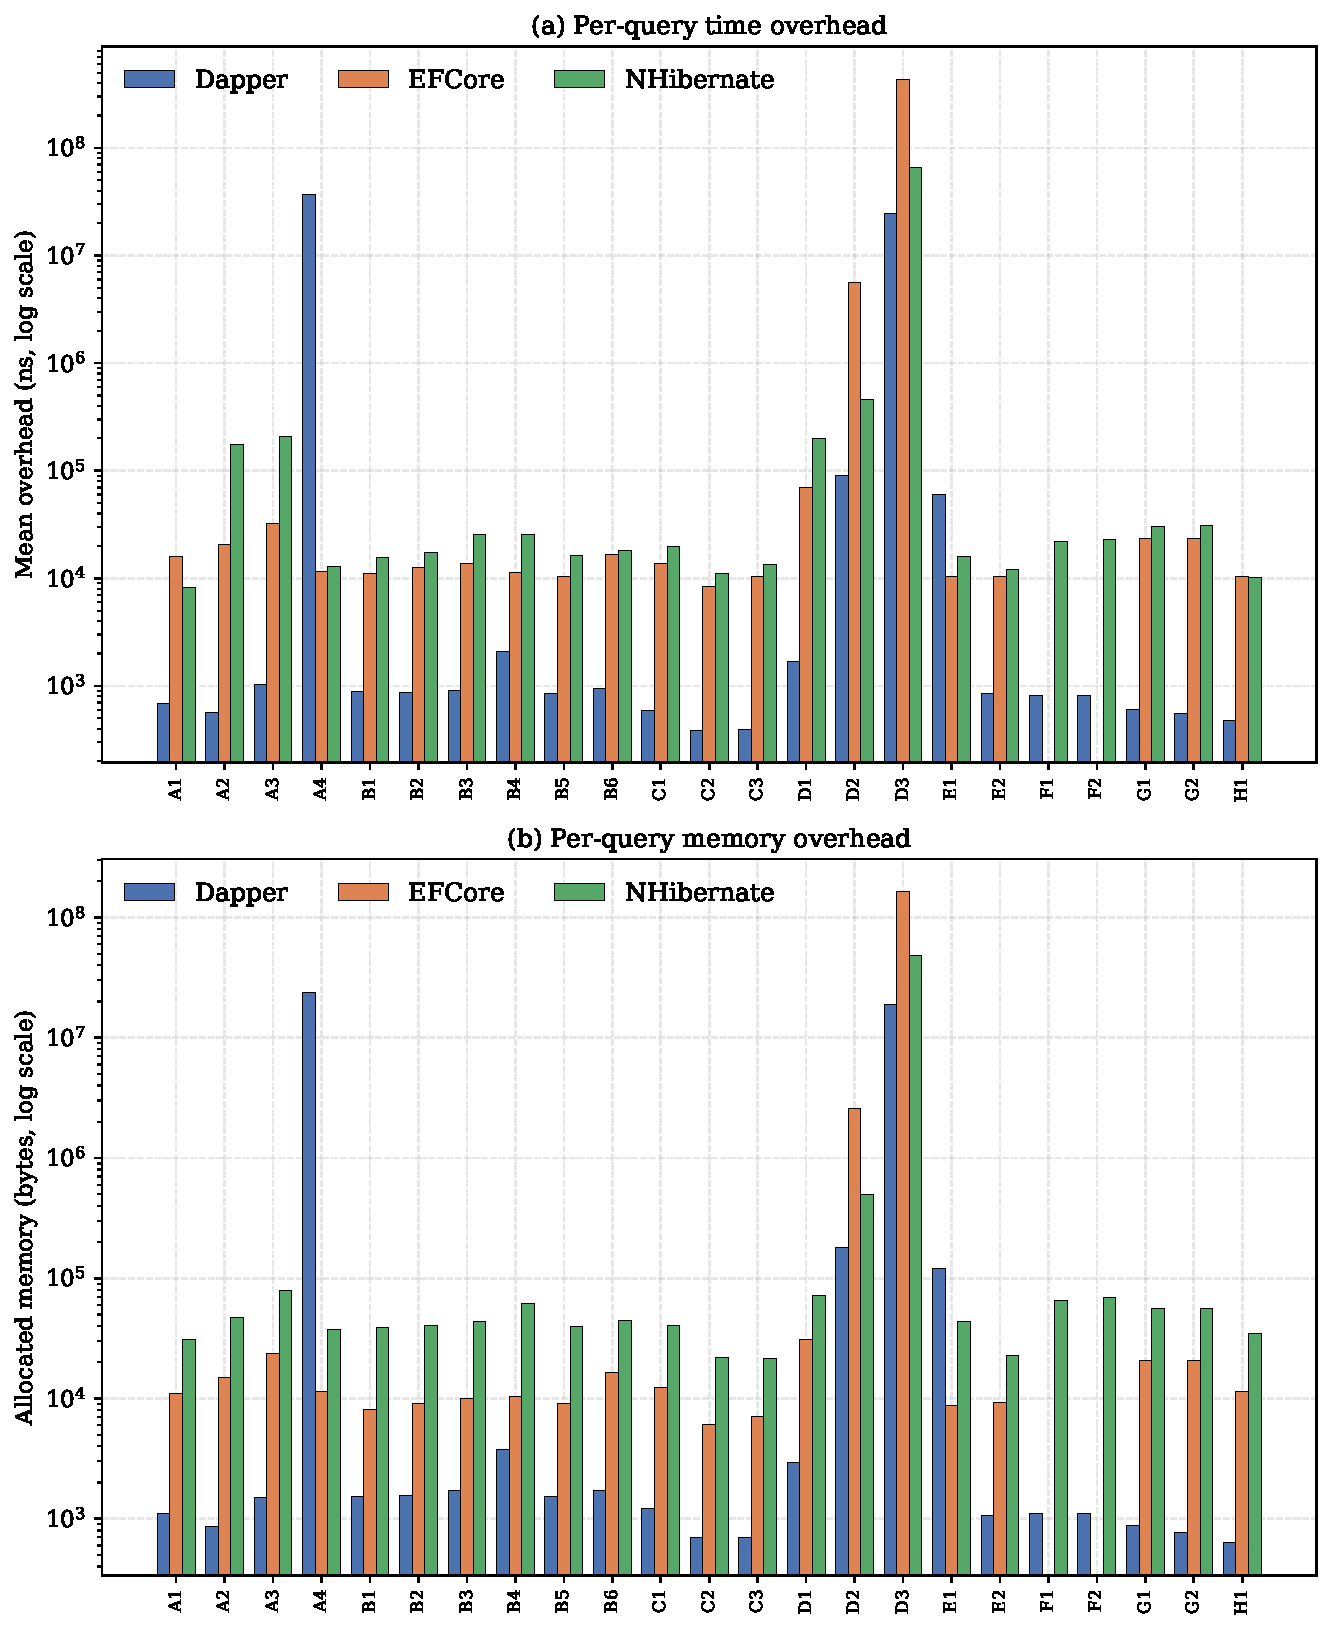
\includegraphics[width=\textwidth]{img/overhead_time_memory.pdf}
\caption[Per-query ORM overhead]{Per-query (a) time overhead and (b) memory overhead with the database mocked, on a logarithmic scale. Dapper is roughly an order of magnitude cheaper than the two full ORMs across the suite. Note the query-shape-dependent anomalies (A4, D2, D3), discussed in the text.}
\label{fig:overhead-time-memory}
\end{figure}

The order-of-magnitude rule has revealing exceptions that only the mocked measurement makes visible, and they all stem from query shape rather than framework identity. The stored-procedure query A4 inverts the ranking: Dapper buffers the full $66{,}741$-row result eagerly --- by default its \texttt{Query} method reads the entire reader into an in-memory list\footnote{\url{https://www.learndapper.com/misc/buffered-unbuffered}} --- spending $36.9$\,ms and allocating $24$\,MB, while the full \acrshort{orm}s stay near $12$\,\textmu s. The optional-relationship query D3 produces the largest cost of the entire study --- EF Core takes $437$\,ms and allocates $164$\,MB. The cause is \emph{data duplication}: eagerly loading an entire table together with a one-to-many navigation in a single query makes EF Core emit a \acrshort{sql} \texttt{JOIN} that repeats every joined-row column across all of its related rows, so the framework transfers and materialises a heavily inflated result set --- the effect that the framework's split-query feature exists to avoid.\footnote{\url{https://learn.microsoft.com/ef/core/querying/single-split-queries}} The many-to-many query D2 shows a milder version of the same effect ($5.6$\,ms, $2.6$\,MB for EF Core). Finally, we dropped EF Core from F1, F2 testing (JSON queries) because of difficulties related to mocking JSON string values in the mocked environment. Nevertheless, Dapper and NHibernate handled them at typical cost, but its important to note that we were only creating mocked string constant values, not the actual JSON data. These cases underline that framework overhead is not a scalar property of a framework but a function of the framework \emph{and} the query.

The contrast with full-database execution is the central result. \Cref{fig:overhead-vs-fulldb} places, side by side, the same five inexpensive queries as measured by Abrahám against a live database (panel a) and by the mocked benchmark here (panel b). Against the database the three frameworks are nearly identical --- A1 takes $750$, $809$, and $742$\,\textmu s for Dapper, EF Core, and NHibernate, a spread under $10\%$ --- because the fixed cost of executing the query dwarfs the mapping cost. If you substract the database, and the same three frameworks diverge by more than $20\times$.

\begin{figure}[H]
\centering
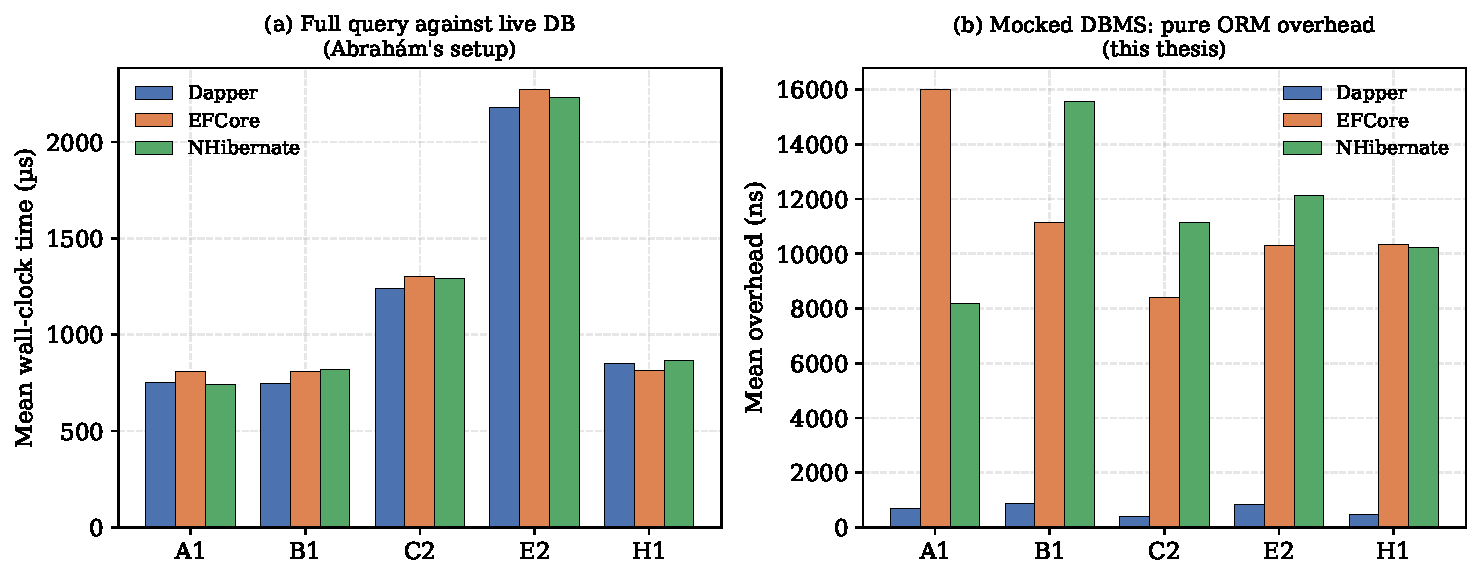
\includegraphics[width=\textwidth]{img/overhead_vs_fulldb.pdf}
\caption[Database execution masks ORM overhead]{The same five inexpensive queries measured (a) end-to-end against a live database (Abrahám's setup~\cite{abrahamFrameworkAgnosticQueryAdaptation2025}, in \textmu s) and (b) with the database mocked to isolate ORM overhead (this thesis, in ns). End-to-end the frameworks are within $\sim$10\%; the database execution masks a $>$20$\times$ difference in pure mapping overhead.}
\label{fig:overhead-vs-fulldb}
\end{figure}

\section{Implications for the Migration Assistant}
\label{sec:overhead-implications}

Three conclusions carry into the rest of the thesis. The migration is performance-significant: moving a query between a micro-ORM and a full \acrshort{orm} can change its framework-attributable cost by an order of magnitude even when the underlying \acrshort{sql} is identical, which is exactly why the assistant preserves query semantics rather than rewriting them and leaves cost-driven choices to an explicit, opt-in advisory step (\cref{chap:future}). Overhead is query-shaped, not framework-shaped: the A4, D2, and D3 anomalies show that any future cost model must be per-query, matching the granularity at which the assistant already operates on queries. And the methodology is reusable: the recording-and-mocking harness is framework-agnostic, so as the assistant grows to treat raw \acrshort{sql} as a first-class source and \acrshort{odm}/\acrshort{ogm} mappings as targets, the same technique can quantify the overhead those new paradigms introduce.

These benchmarks cover only the three .NET source frameworks; the Spring Data MongoDB and Spring Data Neo4j targets were not benchmarked, as the JVM tooling and the very different cost profiles of document and graph stores fall outside the scope of this comparison. Extending the overhead study to the target side is a natural continuation noted in \cref{chap:future}. Even confined to the relational source frameworks, the experiment establishes the quantitative significance against which the LLM assistant's translations are made, and hopefully motivates developers and system/database architects to consider this thesis's main contribution -- a framework-agnostic, semantics-preserving, execution-verifiable, LLM-based translation assistant.